\documentclass[12pt]{beamer}
%\usepackage[margin=1.25in]{geometry}                % See geometry.pdf to learn the layout 
\usepackage{graphicx}
\usepackage{amssymb}
\usepackage{epstopdf}
\usepackage{hyperref}
\usepackage{setspace}
\usepackage{natbib}
\usepackage{booktabs}
\usepackage{amsmath}
\usepackage{caption}
\usepackage{mathtools}

\usepackage{graphicx}
\usepackage[usestackEOL]{stackengine}
\usepackage{xcolor}

\def\calloutsymbigarrow{%
  \ensurestackMath{%
  \scalebox{1.7}{\color{red}\stackunder[0pt]{\bigcirc}{\bigg\downarrow}}}%
}
\newcommand\callouttextbigarrow[1]{%
  \def\stacktype{S}\renewcommand\useanchorwidth{T}\stackText%
  \stackunder{\calloutsymbigarrow}{\scriptsize\Longstack{#1}}\stackMath%
}
\newcommand\calloutbigarrow[3][2.5pt]{%
  \def\stacktype{L}\stackMath\stackunder[#1]{#2}{\callouttextbigarrow{#3}}%
}

\def\calloutsymbig{%
  \ensurestackMath{%
  \scalebox{2.3}{\color{red}\stackunder[0pt]{\bigcirc}{\downarrow}}}%
}
\newcommand\callouttextbig[1]{%
  \def\stacktype{S}\renewcommand\useanchorwidth{T}\stackText%
  \stackunder{\calloutsymbig}{\scriptsize\Longstack{#1}}\stackMath%
}
\newcommand\calloutbig[3][2.5pt]{%
  \def\stacktype{L}\stackMath\stackunder[#1]{#2}{\callouttextbig{#3}}%
}


\def\calloutsym{%
  \ensurestackMath{%
  \scalebox{1.7}{\color{red}\stackunder[0pt]{\bigcirc}{\downarrow}}}%
}
\newcommand\callouttext[1]{%
  \def\stacktype{S}\renewcommand\useanchorwidth{T}\stackText%
  \stackunder{\calloutsym}{\scriptsize\Longstack{#1}}\stackMath%
}
\newcommand\callout[3][1.5pt]{%
  \def\stacktype{L}\stackMath\stackunder[#1]{#2}{\callouttext{#3}}%
}

\def\calloutsymon{%
  \ensurestackMath{%
  \scalebox{1.7}{\color{red}\stackon[0pt]{\bigcirc}{\uparrow}}}%
}
\newcommand\callouttexton[1]{%
  \def\stacktype{S}\renewcommand\useanchorwidth{T}\stackText%
  \stackon{\calloutsymon}{\scriptsize\Longstack{#1}}\stackMath%
}
\newcommand\callouton[3][1.5pt]{%
  \def\stacktype{L}\stackMath\stackunder[#1]{#2}{\callouttexton{#3}}%
}
%\renewcommand\useanchorwidth{T}

\begin{document}
\title{Using machine learning to infer and benchmark firm-firm trading networks}
\author{Jesse Tweedle}
%\date{}

\begin{frame}{}

\maketitle

\end{frame}

\begin{frame}{Broad introduction to machine learning}

\begin{block}{Algorithms that do statistics}
\begin{itemize}
\item Like regular econometrics, but focused on getting $\hat{y}$ right instead of estimating $\hat{\beta}$
\item Mainly classification; e.g., optical character recognition (``what letter is this?")
\item Converted to regression-style question:
\begin{itemize}
\item One observation = one image of a character
\item Dependent variables = each pixel in the image
\item Predict what the letter is (e.g., $\hat{y} $ = `a')
\end{itemize}
\end{itemize}
\end{block}

\end{frame}

\begin{frame}{Example: image recognition}

\begin{figure}[h]
\caption{A three. A prediction algorithm should produce $\hat{y} = 3$.}
\centering
\fbox{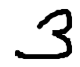
\includegraphics[width=0.75\textwidth]{three}}
\end{figure}

\end{frame}

\begin{frame}{Why ``learning''?}

\begin{block}{Easy reason---it does variable selection}

Problem: you get firm data from CRA, you want to assign a NAICS code ($y$). 

\begin{itemize}
\item There are tons of possible variables you could use to predict a firm's industry.
\item Possibly more variables than observations (which means can't solve OLS problem $(X^T X)^{-1} X^T y$
\end{itemize}

\end{block}

\begin{block}{ML approach}
Stick all the variables in a blender
\begin{itemize}
\item Algorithm starts with no predictors, adds them one-by-one 
\item ``Learns'' which ones are most important 
\item Use those coefficients to predict industries for out-of-sample firms
\end{itemize}

\end{block}

\end{frame}

\begin{frame}{Some links / resources}

\begin{block}{Google's Open Source AI: TensorFlow}
\begin{itemize}
\item \url{https://github.com/tensorflow/tensorflow}
\item \url{https://www.tensorflow.org/}
\item \url{http://playground.tensorflow.org/}
\end{itemize}
\end{block}

\begin{block}{Facebook / Columbia / World Bank datasets}
Analyze satellite imagery to create dataset on building density
\url{https://code.facebook.com/posts/596471193873876/open-population-datasets-and-open-challenges/}
\end{block}

\begin{block}{Text: Elements of Statistical Learning}
Hastie, Tibshirani, Friedman (2009)
\url{http://statweb.stanford.edu/~tibs/ElemStatLearn/}
\end{block}

% visualization stuff

% "statistical learning" books. 

% tensorflow, others.

\end{frame}

%\begin{frame}{Outline}
%\begin{enumerate}
%\item Problem
%\item Needs
%\item Approach: separate data, benchmarking, methods steps, improve each one separately.
%\item Data sources
%\item Methods
%\item Results
%\end{enumerate}
%\end{frame}

\begin{frame}{Problem}

\begin{block}{Goal: study firm-firm trade}
To understand
\begin{itemize}
\item supply chains and vertical integration
\item intra-firm trade
\item and more
\end{itemize}
\end{block}

\begin{block}{Problem: we don't have firm-firm transaction data}
But: 
\begin{itemize}
\item we have lots of useful data
\item and an idea of how to use it
\end{itemize}
\end{block}

%Have lots of data. Want to infer firm-firm trading relationships. But: want it to be internally consistent---a firm can't produce \$10 million of output and only have customers that buy \$1,000. Also need it to be externally consistent: if you add up all the firm-firm relationships, you should get back to industry accounts. More detail on this later.

\end{frame}

\begin{frame}{Facts / needs}
% this slide: some things: few relationships. 
\begin{block}{Facts: start with manufacturing}
\begin{itemize}
\item $\approx 30$k plants. 
\item $\approx 900$m possible connections.
\item $\approx 70$ industries (IOIC)
\item $\approx 200+$ goods (detailed confidential IOCC)
\end{itemize}
\end{block}

\begin{block}{Needs}
\begin{itemize}
\item Data that indicates relationship between plants
\item Method to identify / predict relationships: typical application of machine learning
\item Method to benchmark to make sure it all adds up: unusual application of machine learning
\end{itemize}
\end{block}

\end{frame}



\begin{frame}{Normal approach: idea}

\begin{block}{To achieve this:}
\begin{itemize}
\item Data that indicates relationship between plants
\item Method to identify relationships
\end{itemize}
\end{block}

\begin{block}{Do this:}
\begin{itemize}
\item Use supply-use/input-output tables
\item Assume every firm-firm relationship is the same as the industry IO relationship
\end{itemize}
\end{block}

\end{frame}

\begin{frame}{Normal approach: problems}

% use full thing here, or just manufacturing?
\begin{block}{Implies way too many plant-plant relationships}
\begin{itemize}
\item Use goods-only, square IO table, DC level
\item $\approx 70^2 = 4900$ possible connections
\item $\approx $ actual connections
\item 50\% density---half of the possible connections are given
\item Gets worse using full table: 90\% density of $50000+$ possible connections
\end{itemize}
\end{block}

% HERE: why is this wrong.

% every plant in an industry trades with every other plant in the other industry (with positive entry in IO table)
% if industries are the same, then plant trades with itself---wrong

% To get an idea of better number. Just use ASM commodity files. Commodities just don't line up.
% Can't just cut IO table off at some direct requirement level either, because you drop so much expenditure.


\end{frame}

\begin{frame}{Normal approach: problems}

% assign small plant as important supplier to big plant---IO numbers are not consistent with plant numbers
% may be missing some connections? industry definitions or something.
% so still need to benchmark.

\begin{block}{Plant and IO data may not be consistent}
\begin{itemize}
\item Relationship may not be consistent with plant data; some plants may export more or less, some plants may import more or less % may be assigning tiny auto parts plant as an important supplier to GM assembly plant
\item Plant-plant relationships may not be consistent with industry IO
\end{itemize}
\end{block}


\begin{block}{Problems: summary}
\begin{itemize}
\item Don't correctly identify the links
\item And still need to benchmark anyway
\end{itemize}
\end{block}

\end{frame}


\begin{frame}{Machine learning approach}

\begin{block}{Step 1. Data}
Use lots, from many sources.
\end{block}

\begin{block}{Step 2. Identify / predict connections}
\begin{itemize}
\item Typical, statistical, ``classification'' application of machine learning. 
\item For a possible firm-firm pair $(i,j)$, predict whether there is a link or not. 
\end{itemize}
\end{block}

\begin{block}{Step 3. Benchmark (solving a huge linear programming problem)}
\begin{itemize}
\item Unusual application of machine learning.
\item Quick, cheap, accurate way to solve \emph{sparse} system of equations.
\end{itemize}
\end{block}

\end{frame}


\begin{frame}{Step 1. Data}

For now, stick to one year, 2010. Easier on classifications / concordances / consistency across datasets. 

\begin{itemize}
\item Surface Transportation File (STF): database of goods shipments; commodity, value, distance, postal code origin and destination
\item ASM: industry, postal codes, provincial shipment breakdown, commodity inputs and outputs
\item Input-output tables (IO): industry, commodity inputs and outputs; can calculate industry pair expenditures and direct requirements
\item Inter-provincial trade flows (IPTF): trade by province origin and destination, and commodity
%\item IER (later)
\end{itemize}

% 

\end{frame}

\begin{frame}{Step 2. Identify / predict connections}

\begin{block}{Want regular (logistic) regression form.}
Write $y_{ij}=\mathbf{1} \{ \text{firm $i$ buys from firm $j$}  \} $, %an indicator for whether or not there is a directed link between $i$ and $j$.
Estimate:
\[ P( y_{ij} = 1 | X_{ij}) \]
\end{block}

\begin{block}{What is in $X_{ij}$?}
\begin{itemize}
\item Entry in industry IO table or IPTF
\item STF shipment from $j$'s postal code to $i$'s postal code
\item $j$ exports to $i$'s province
\item Entry in plant IO table defined by ASM commodity data
\item Is there another possible producer of that good in the area of $j$, or another consumer in the area of $i$?
\item Combinations of all of the above, et cetera
\end{itemize}
\end{block}

%\begin{block}{$y_{ij}$ is indicator for whether a firm pair $ij$ has a link.}
%\[ y_{ij} = \mathbf{1} \{ \text{firm $i$ buys from firm $j$} \} \]
%\end{block}
%
%\begin{block}{$X_{ij}$ are characteristics that may define a relationship between $i$ and $j$}
%\end{block}

% create potential firm pairs
% then get data for pairs based on what we think connections will be, geography, IO, IPTF, ASM, STF, etc.
% then use some algorithm to get beta
% then use some cutoff to classify
% work in progress.

\end{frame}

\begin{frame}{Step 2. Identify / predict connections}

\begin{block}{Solve problem}
\begin{itemize}
\item This is classification problem: does the link exist (classify `yes'), or not (classify `no')
\item Many algorithms for this; I broadly divide into ``things I understand" (all very similar to econometrics) and ``deep learning'' (e.g., neural networks). % black boxes. TensorFlow e.g., deep learning is used for image classification, AI that goes in Google / Tesla's self driving cars, one guy comma.ai built his own. all open sourced now, TensorFlow, keras, etc.
% the bottleneck / scarce resource is talent, not the software  hardware. so they open source hardware (e.g., Fbook's open source server designs) and software (everything open sourced on github, for anyone to use and/or copy)
%\item Will use LASSO (glmnet package in R) here
\item Called ``supervised learning'' because we know the things we want to predict, so we ``supervise'' the algorithm until it does what we want (predict firm-firm links).
\end{itemize}
\end{block}

\begin{block}{Predict links $\hat{y}_{ij}$}
And use them as input into next step. (Still a work in progress. For now, I'll focus on benchmarking bit.)
\end{block}

%\begin{itemize}
%\item Use machine learning algorithm to solve problem
%\item Use solution to predict links $\hat{y}_{ij}$.
%\item 
%\end{itemize}

\end{frame}

\begin{frame}{Step 3. Benchmark}

% here I"ll spend most of my time.
\begin{block}{Have links, but need to benchmark: }
\end{block}

\begin{block}{To make internally consistent}
\begin{itemize}
\item E.g., a plant that produces \$1m in output and is the only supplier to a plant that buys \$10m in intermediates---firm data not consistent with each other.
\end{itemize}
\end{block}

\begin{block}{To make externally consistent}
\begin{itemize}
\item Want the implied expenditure between industries to match the industry totals from the IO tables
\end{itemize}
\end{block}


\end{frame}


\begin{frame}{Benchmark application}

\begin{block}{Benchmarking is a big linear program}
We want to make sure everything adds up to national accounts by solving a bunch of equations. But! We have an underdetermined system, too many parameters and not enough equations.
\end{block}

\begin{block}{Another but!: Recall we want firm-firm network to be sparse}
Donoho and Tsaig (2008): if the solution to linear program is sparse, we can use $\ell$-1 minimization (LASSO) to solve the program quickly
\end{block}

%Intead of using this for statistics / machine learning problems, we use it to solve sparse, underdetermined linear programming problem.


\end{frame}


%\begin{frame}{Methods}
%
%(1) Use IO, STF, ASM, IPTF to give any possible link between firms (e.g., an upper bound on links between firms), then a subset that we think is most likely (a lower bound on the set of links between firms).
%
%(2) Benchmark to make expenditures between firms internally and externally consistent. Need to solve a huge, underdetermined system of equations, a big linear programming problem (tens-of-thousands of equations, hundreds of millions of parameters, maybe). Lasso is a good way.
%
%\end{frame}


\begin{frame}{LASSO}

\begin{block}{Definition}
\begin{itemize}
\item Least absolute shrinkage and selection operator (Tibshirani 1996)
\item Just like OLS, plus an extra parameter that defines the ``penalty''
\item Can solve problems with more coefficients than observations (or in our case, more unknowns than equations)
\end{itemize}
\end{block}

\begin{block}{Penalty}
\begin{itemize}
\item Penalty helps to select important parameters by shrinking less important ones to zero
\end{itemize}
%Idea: penalize the coefficients, so the solution is ``better'' if each $\beta_k$ is smaller. $\lambda$ determines how important the penalty is, relative to getting the solution right. 
\end{block}

% pros: can solve underdetermined problems, more coefficients than observations, beta longer than y. fast, relative to LP solvers (I think?)
% cons: needs algorithm, instead of closed-form like OLS

\end{frame}

\begin{frame}{OLS / LASSO: very similar problems}

\begin{block}{OLS}
\begin{equation}
\min_{\beta}  \sum_i \left( y_i - X_i \beta \right)^2
\end{equation}
\end{block}

\begin{block}{LASSO}
\begin{equation}
\min_{\beta}  \sum_i \left(y_i - X_i \beta \right)^2 + \overbrace{\lambda \sum_k | \beta_k |}^{\text{Penalty}}
\end{equation}
\end{block}

Next, get the equations we need to benchmark, and then translate them into a form we can use.

\end{frame}

\begin{frame}{Benchmark application}

% want links between firms and regions, $a_{ri}$, and firm-firm links $g_{ji}$
% expenditure shares.
%Have several sets of benchmarking equations:

%need lots of notation.

%\[ K \callout{\subseteq}{by compactness} \bigcup_{J=1}^{n} V_{nJ} \]
%
%\[ \lim_{n\rightarrow \infty} \int\limits_{x} f_{n} \mathrm{d}\mu 
%\callout[1.8pt]{=}{By Monotone\\Convergence Theorem} \int\limits_{x} f \mathrm{d}\mu
%\]

\begin{block}{Firm sales to all customers add up to total sales; $N$ equations.}
\begin{equation}
%\sum_r a_{ri} s_i + \sum_j \underbrace{g_{ji}}_{$j$'s share of expenditure on $i$} s_j = s_i, \forall i=1,\ldots,N
\sum_r \callout[1.8pt]{a_{ri}}{$r$'s share of\\ expenditure on $i$} \callouton[1.8pt]{M_r}{Region $r$'s\\ total expenditure} + \sum_j (1-\callouton[1.8pt]{\beta_i}{$i$'s value\\ added share}) \callout[1.8pt]{g_{ji}}{$j$'s share of\\ expenditure on $i$} s_j = \callouton[1.8pt]{s_{i}}{sales of firm $i$}, \forall i=1,\ldots,N
\end{equation}
\end{block}

%\begin{equation}
%%\sum_r a_{ri} s_i + \sum_j \underbrace{g_{ji}}_{$j$'s share of expenditure on $i$} s_j = s_i, \forall i=1,\ldots,N
%\sum_r \overbrace{a_{ri}}^{\mathclap{\text{$r$'s share of expenditure on $i$}}} s_i + \sum_j \underbrace{ \left( ? \right) }_{\mathrlap{\text{what is this?}}} s_j = s_i, \forall i=1,\ldots,N
%\end{equation}

\end{frame}

\begin{frame}{Benchmark application}

\begin{block}{Firm expenditures on all other firms add up to total expenditures; same for regions. $R+N$ equations.}
\begin{gather}
\sum_j (1-\beta_i) \callouton[1.8pt]{g_{ij}}{$i$'s share of\\ expenditure on $j$} s_i = (1-\beta_i) s_i, \forall i=1,\ldots,N \\
\sum_i a_{ri} M_r = \callout[1.8pt]{M_r}{Region $r$'s\\ total expenditure}, \forall r=1,\ldots,R
\end{gather}
\end{block}

\end{frame}

\begin{frame}{Benchmark application}

\begin{block}{Firm expenditures on all other firms within industry pairs add up to industry pair expenditure from IO table; $K^2$ equations.}
\begin{gather}
\underbrace{\sum_{i \in k} \sum_{j\in k'}}_{\mathclap{\text{all firm pairs in $(k,k')$}}} \overbrace{(1-\beta_i) g_{ij} s_j}^{\mathclap{\text{$j$'s expenditure on $i$}}} = \calloutbig[1.8pt]{S_{kk'}}{Total expenditure of \\industry $k$ on industry $k'$}, \forall \text{ industry pairs }(k, k') 
\end{gather}
\end{block}

\end{frame}

\begin{frame}{Benchmark application}

\begin{block}{Size of problem}
\begin{itemize}
\item Unknowns: RN region-firm shares $(a_{11},\ldots,a_{RN})$ and $N^2$ firm-firm shares $(g_{11},\ldots,g_{NN})$
\item Equations: $N$ firm sales, $N$ firm expenditure, $R$ region expenditure, $K^2$ industry pair expenditure
\item Number of unknowns much bigger than number of equations \[(R+N)N >> 2N + R + K^2\] 
\item E.g., for $N\approx 30,000$ plants, $R \approx 70$ ERs, $K \approx 200$ industries, unknowns almost 900 million, equations around 100,000 % almost 1000 times more unknowns. 
\end{itemize}
\end{block}

\end{frame}

\begin{frame}{Benchmark application}

\begin{block}{Rewrite these equations into matrix form for input into algorithm}
\begin{equation}
\callout[1.8pt]{X}{known parameters on\\ LHS of equations} \callouton[1.8pt]{y}{unknown vectors $a$ and $g$ all stuck together}=\calloutbigarrow[1.8pt]{c}{known parameters \\on RHS of equations}
\end{equation}
\end{block}

\begin{block}{Algorithm solves for parameters $y$}
Many details. To translate to regression notation, $X$ is $X$ (characteristics), $y$ is $\beta$ (parameters), $c$ is $y$ (outcomes). %All in levels, so more likely to match large firms, industry pairs and regions, which is important for benchmarking. %(I.e., more likely to match national accounts overall than every individual plant pair.)
\end{block}

\end{frame}


% Results:
% It solves the problem, and pretty quickly.
% Results: do the parameters make sense? do firm sales match? expenditures?
% Industry pairs? err, skip that bit. work in progress. Or, because they don't work too well,
% that says the link prediction bit needs more work. Also, imports / exports. 

% conclusion: methods work well. Problems in solution point to places that need improvement.

% fake results, to make sure it works.

\begin{frame}{Results}

\begin{block}{To start, fake results to make sure it works}
Generate economy with regions, firms and industries. See if the algorithm can solve the equations.
\end{block}

\begin{block}{Code available}
For generating fake data, converting equations into the correct form, and analysis:
\url{https://github.com/tweed1e/firm-network-lasso}
\end{block}

\end{frame}

\begin{frame}{Results---fake data}

\begin{block}{Timing}
$N = 15000$, $R=70$, $K=70$, with 1\% firm-firm density; around 200m parameters, 2m of which are nonzero.
\begin{itemize}
\item $\approx 5$ minutes on laptop
\end{itemize}
\end{block}

%\begin{block}{}
\begin{table}[]
\centering
\footnotesize
\caption{\% difference between predicted and actual values}
\label{my-label}
\begin{tabular}{l rrrrr}
\toprule
                          & Obs & Mean &  25$^{th}$ & Median & 75$^{th}$ \\
\midrule                          
Firm sales                 	&	15000	&	$-$0.003	&	$-$0.004	&	$-$0.003	&	$-$0.002	                 \\
Firm exp.           	&	15000	&	0.200	&	$-$2.660	&	$-$0.023	&	2.825	                \\
Industry pair exp. 	&	4900	&	0.000	&	$-$0.930	&	$-$0.006	&	0.841	                 \\
Region exp.         	&	70	&	0.000	&	0.000	&	0.000	&	0.000	                 \\
	\bottomrule
\end{tabular}
\end{table}
%\end{block}

\end{frame}

\begin{frame}{Results---fake data}

\begin{figure}[h]
\caption{Predicted expenditure shares vs. firm size (random sample of 500 firms). All should be equal to 1. Note increase in accuracy as size increases.}
\centering
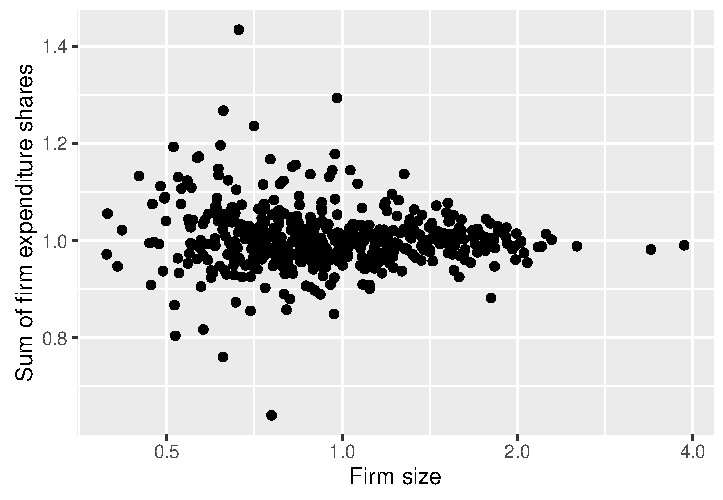
\includegraphics[width=0.8\textwidth]{size-share-plot}
\end{figure}

\end{frame}

%\begin{frame}{Results---real data}
%
%\begin{block}{Timing}
%$N = $, $R=73$, $K=$, with $x\%$ plant-plant density; around 900m parameters, about 10m of which are nonzero.
%\begin{itemize}
%\item $\approx x$ minutes
%\end{itemize}
%\end{block}
%
%%\begin{block}{}
%\begin{table}[]
%\centering
%\footnotesize
%\caption{\% difference between predicted and actual values}
%\label{my-label}
%\begin{tabular}{l rrrrr}
%\toprule
%                          & Obs & Mean &  25$^{th}$ & Median & 75$^{th}$ \\
%\midrule                          
%Plant sales                 	&		&		&		&		&		                 \\
%Plant expenditure           	&		&		&		&		&		                \\
%Industry pair exp. 	&		&		&		&		&		                 \\
%Region exp.         	&		&		&		&		&		                 \\
%	\bottomrule
%\end{tabular}
%\end{table}
%%\end{block}
%
%\end{frame}

\begin{frame}{Results---real data}

Fig: firm size, and maybe expenditure. And next frame: industry.

%\begin{figure}[h]
%\caption{Predicted firm output vs. actual firm output (figure is placeholder).}
%\centering
%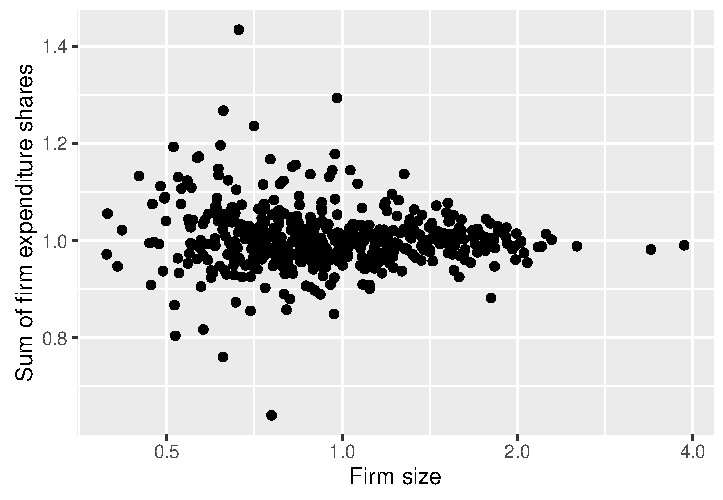
\includegraphics[width=0.8\textwidth]{size-share-plot}
%\end{figure}

\end{frame}

\begin{frame}{Conclusion---benchmarking algorithm}

\begin{block}{On fake data}
\begin{itemize}
\item Works well, and fast
\end{itemize}
\end{block}

%\begin{block}{On real data, without industries}
%\begin{itemize}
%\item Works well, and fast
%\item Because it doesn't have too many constraints
%\end{itemize}
%\end{block}

\begin{block}{On real data}
\begin{itemize}
\item Works fast, but so-so accuracy
\item Not surprising, given lack of trade data
\item More importantly: means input data and prediction algorithm needs work; not getting the right industry connections / values
\end{itemize}
\end{block}

%actual: works well, until you add industry expenditures. which means I need to refine the input data, redo the prediction algorithm, and so on.

%good news: the benchmark algorithm works if the input data works. actually surprising it works at all without trade data.

\end{frame}


%\begin{frame}{Results}
%
%Todo: IER to add trade, final demand.
%
%(1) it works, doesn't crash the server (for now).  (2) it's relatively fast (x mins to solve manufacturing problem. (3) it works, relatively well, needs more refinement in input data to get it to work better---import/export registry, IO tables, final demand and such.
%
%\end{frame}

%\bibliographystyle{chicago}
%\bibliography{inferring-firm-networks-2}

\end{document}








